\section{Results}\label{results}

This section reports results in five stages: (1) FE-OLS estimates for
the S\&P~500 panel, (2) DoubleML PLR estimates for sentiment and news
treatments, (3) the intraday price high specification, (4) robustness
checks including the placebo test and lag structure analysis, and (5)
the Russell 3000 cap-group analysis.

\subsection{Fixed-Effects OLS: S\&P 500
Panel}\label{fixed-effects-ols-sp-500-panel}

Table~\ref{tab:fe_ols} reports the four
FE-OLS specifications. The primary result is unambiguous:
\texttt{twitter\_sent} is statistically insignificant in all four
models, and its coefficient does not change appreciably when the full
confounder matrix is added.

Model~1, the baseline regression of \texttt{return} on
\texttt{twitter\_sent} with firm fixed effects only, produces a
coefficient of \(- 0.370\) (SE \(= 0.230\), \(p > 0.10\)). The \(R^{2}\)
of 0.002 confirms that Twitter sentiment alone explains essentially none
of the within-firm variation in intraday returns. Model~2 adds the full
control vector; the \texttt{twitter\_sent} coefficient moves to
\(- 0.422\) (SE \(= 0.325\)) and remains insignificant. The \(R^{2}\)
rises to 0.019, driven primarily by two significant controls: news
sentiment (\texttt{news\_sent} \(= - 1.056\), \(p < 0.01\)) and the
30-day RSI (\texttt{rsi\_30} \(= + 0.084\), \(p < 0.01\)). The negative
news sentiment coefficient indicates that a one-unit increase in the
Bloomberg daily news sentiment score is associated with a \(- 1.06\)
cent same-day return within firms, a substantially larger and more
reliably estimated effect than the Twitter channel. The positive RSI
coefficient is consistent with short-term price momentum: firms on an
upward 30-day trajectory tend to continue gaining within the trading
day.

Models~3 and~4 test alternative treatment constructions. The
negative-clipped measure (\(\text{min}(\text{twitter\_sent},0)\),
Model~3) produces a coefficient of \(- 0.072\) (SE \(= 0.271\)), smaller
in absolute value than the unrestricted measure in Model~1, suggesting
that the negative tail of Twitter sentiment is not a disproportionately
powerful predictor relative to the full sentiment distribution. Model~4,
using \texttt{twitter\_neg\_count} following Teti et al.\ (2019), yields a coefficient of
\(+ 0.000533\) (SE \(= 0.000971\)), not significant. The positive sign
is consistent with the hypothesis that high tweet volume---even
predominantly negative volume---signals elevated attention rather than
bearish information, but the effect is economically trivial and
statistically indistinguishable from zero.

\subsection{DoubleML Estimates: Twitter and News
Sentiment}\label{doubleml-estimates-twitter-and-news-sentiment}

Table~\ref{tab:dml_twitter} and
Table~\ref{tab:dml_news} report the
DoubleML PLR estimates. The contrast with the FE-OLS results is
substantial.

\textbf{Twitter sentiment.} The PLR estimate for \texttt{twitter\_sent}
is \(- 0.924\) (SE \(= 0.226\), \(p < 0.01\)), statistically significant
at the 1\% level. This coefficient survives 20 repetitions of 5-fold
cross-fitting and is stable across bootstrap draws, indicating it is not
an artifact of a particular fold partition. The negative sign implies
that higher Twitter sentiment is associated with a lower open-to-close
return on the same day, after nonparametrically partialling out the full
confounder vector. Economically, a one-standard-deviation increase in
\texttt{twitter\_sent} (\(\sigma \approx 0.165\)) is associated with a
reduction of approximately \(0.15\) cents in the same-day return---a
modest magnitude given that the average absolute intraday return in the
sample is approximately \(2.14\)\%.

The \texttt{twitter\_neg\_count} specification
(Table~\ref{tab:dml_twitter},
column~2) yields a coefficient of \(+ 0.003987\) (SE \(= 0.001503\),
\(p < 0.01\)), significant and positive. This sign reversal relative to
the continuous sentiment measure is notable. A higher count of
negative-polarity tweets is associated with a slightly higher same-day
return. One interpretation is that a surge in negative tweets reflects
elevated attention to the firm---perhaps controversy or an emerging news
event---which temporarily raises demand from retail traders responding
to salience rather than to the negative content of the messages. This
interpretation is speculative and would require an instrument separating
attention from sentiment quality to test rigorously.

\textbf{News sentiment.} The PLR estimate for \texttt{news\_sent} is
\(- 0.759\) (SE \(= 0.135\), \(p < 0.01\)), consistent in sign with the
FE-OLS Model~2 result and precisely estimated. News sentiment is the
stronger and more consistently identified treatment across both
specifications. The convergence between the FE-OLS and DoubleML
estimates for news sentiment (\(- 1.056\) vs. \(- 0.759\)) is
reassuring, suggesting that the linear OLS approximation performs
reasonably well for the news channel, where the relationship between
sentiment and return is likely more direct (news-driven price moves are
well-documented) and less susceptible to nonlinear confounding.

\subsection{Intraday Price High as
Outcome}\label{intraday-price-high-as-outcome}

Table~\ref{tab:dml_pxhigh} reports
DoubleML estimates where \texttt{px\_high} (the intraday high price)
replaces \texttt{return} as the dependent variable. The
\texttt{twitter\_sent} coefficient is \(+ 1.610\) (SE \(= 0.217\),
\(p < 0.01\))---positive and larger in magnitude than the
\texttt{return} estimate. The sign flip is striking: positive sentiment
is associated with a \emph{higher} intraday price ceiling but a
\emph{lower} close-to-open return. The \texttt{twitter\_neg\_count}
coefficient on \texttt{px\_high} is \(- 0.002082\) (\(p < 0.10\)), again
opposite in sign to the \texttt{return} specification.

A consistent interpretation is that positive Twitter sentiment generates
early-session buying pressure---pushing the intraday high upward---which
is subsequently mean-reverted by informed sellers or algorithmic
liquidity provision before the close. This dynamic is consistent with
noise-trader-driven intraday reversals documented in the market
microstructure literature and with the reverse causality evidence
discussed in Section~\ref{robustness-checks}:
sentiment may amplify short-lived price moves that do not persist to the
daily close. It also suggests that the Bloomberg daily sentiment
average, aggregating pre-market and intraday tweets, may be
contemporaneous with or lagging intraday price action rather than
leading it.
This sign pattern --- positive sentiment lifts the intraday ceiling but not the daily close --- is revisited in Section~\ref{discussion} as additional evidence that the Bloomberg daily sentiment aggregate is contemporaneous with, rather than leading, intraday price action.

\subsection{Robustness Checks}\label{robustness-checks}

\textbf{Placebo test.} The placebo regression of yesterday's return
(\texttt{lag1}) on today's Twitter sentiment within firms produces a
coefficient of \(+ 2.348\) (SE \(= 0.225\), \(p < 0.01\)). This estimate
is more than twice the magnitude of the forward DoubleML estimate
(\(- 0.924\)). Under the null of no reverse causality, the placebo
coefficient should be indistinguishable from zero. The large,
significant positive value indicates that firms experiencing high
returns today tend to generate more positive Twitter sentiment
tomorrow---a direction of causality running from prices to social media,
not the reverse. This is a serious qualification on the causal
interpretation of all forward-looking estimates in this paper. It does
not rule out that sentiment has some forward predictive content, but it
establishes that the correlation between sentiment and returns is
substantially contaminated by reverse causality.

\textbf{No-reversal test.} When the five sentiment lags (1, 2, 3, 5, 7)
are entered jointly in a fixed-effects regression, none is statistically
significant and the signs alternate. This result is inconclusive: the
lack of significance at lag~1 suggests either that any causal signal is
too weak to survive the multicollinear joint estimation, or that the
lags jointly absorb a sentiment signal that manifests only in isolation.
The result does not support the finding that lag~1 uniquely predicts
returns in a multi-lag specification as found in the original Gu\& Kurov
study.

\textbf{Lag decay.}
Table~\ref{tab:lag_decay} reports
univariate DoubleML estimates at each lag. All ten estimates (five lags
\(\times\) two treatments) are highly significant (\(p < 0.001\)) and
negative, with no monotone decay to zero across lags~1 through~7. The
\texttt{twitter\_sent} coefficients range from \(-1.215\) at lag~1 to
\(-0.674\) at lag~7; significance is sustained throughout with no lag
producing an estimate near zero. This pattern is inconsistent with a
sentiment-causes-price hypothesis, under which one would expect a large
coefficient at lag~1 decaying to insignificance by lag~5 or~7. Persistent
significance across all lags is instead consistent with a common
factor---possibly prior price performance---simultaneously driving both
lagged sentiment (through the reverse causality channel) and current
returns (through momentum). The
lag decay evidence reinforces the placebo finding.

\textbf{Impact persistence.}
Table~\ref{tab:impact_persist}
reports estimates of current sentiment on future returns at leads~1
through~7. \texttt{twitter\_sent} is insignificant at every lead
(\(p > 0.60\) in all cases), confirming that same-day Twitter sentiment
carries no recoverable predictive content for returns over the following
week. \texttt{news\_sent} is significant at leads~1, 2, 3, 5, and~7 but
with alternating signs, suggesting that news sentiment does not predict
future returns in a monotone direction. The sign instability in
\texttt{news\_sent} is consistent with event-specific news that drives
returns in both directions depending on content (e.g., a regulatory
announcement versus an earnings beat), neither of which tips the daily
sentiment score strongly enough to produce a directional signal.

\subsection{Temporal Analysis: S\&P
500}\label{temporal-analysis-sp-500}

Table~\ref{tab:gk_fmb_annual}
and
Figures~\ref{fig:gk_temporal_annual}--\ref{fig:gk_temporal_monthly}
report Fama-MacBeth coefficient estimates on
\texttt{twitter\_sent\_lag1} for each calendar year from 2016 through
early 2026. No year produces a statistically significant estimate. The
coefficients range from \(- 0.326\) (2020) to \(+ 0.249\) (2021) with
standard errors that dwarf the point estimates in most years. The null
result is stable across annual, quarterly, and monthly window
granularities.

This finding has a direct bearing on the interpretation of , whose
sample spans January 2015 to February 2017. The years 2016 and 2017 in
the present sample---the period most closely overlapping with their
data---produce FMB coefficients of \(+ 0.007\) and \(- 0.022\), both
insignificant. There is no evidence of a significant Twitter sentiment
effect in those years on the S\&P~500 universe. The most likely
explanation is that the Bloomberg sentiment measure and the commercial
dataset used by differ in coverage, construction, or the population of
tweets included, so the samples are not directly comparable even over
the same calendar period.

The long-short strategy on the S\&P~500 extended panel
(Table~\ref{tab:gk_ls_annual})
yields positive annualized returns in nine of ten complete years, with
Sharpe ratios ranging from \(- 0.05\) (2024) to \(2.04\) (2023). The
strategy performance is notably heterogeneous and does not exhibit a
consistent time trend. As discussed in
Section~\ref{discussion}, the positive long-short
performance coexisting with insignificant FMB coefficients suggests the
strategy captures cross-sectional dispersion in realized returns rather
than the lagged sentiment signal.

\begin{figure}[htbp]
\centering
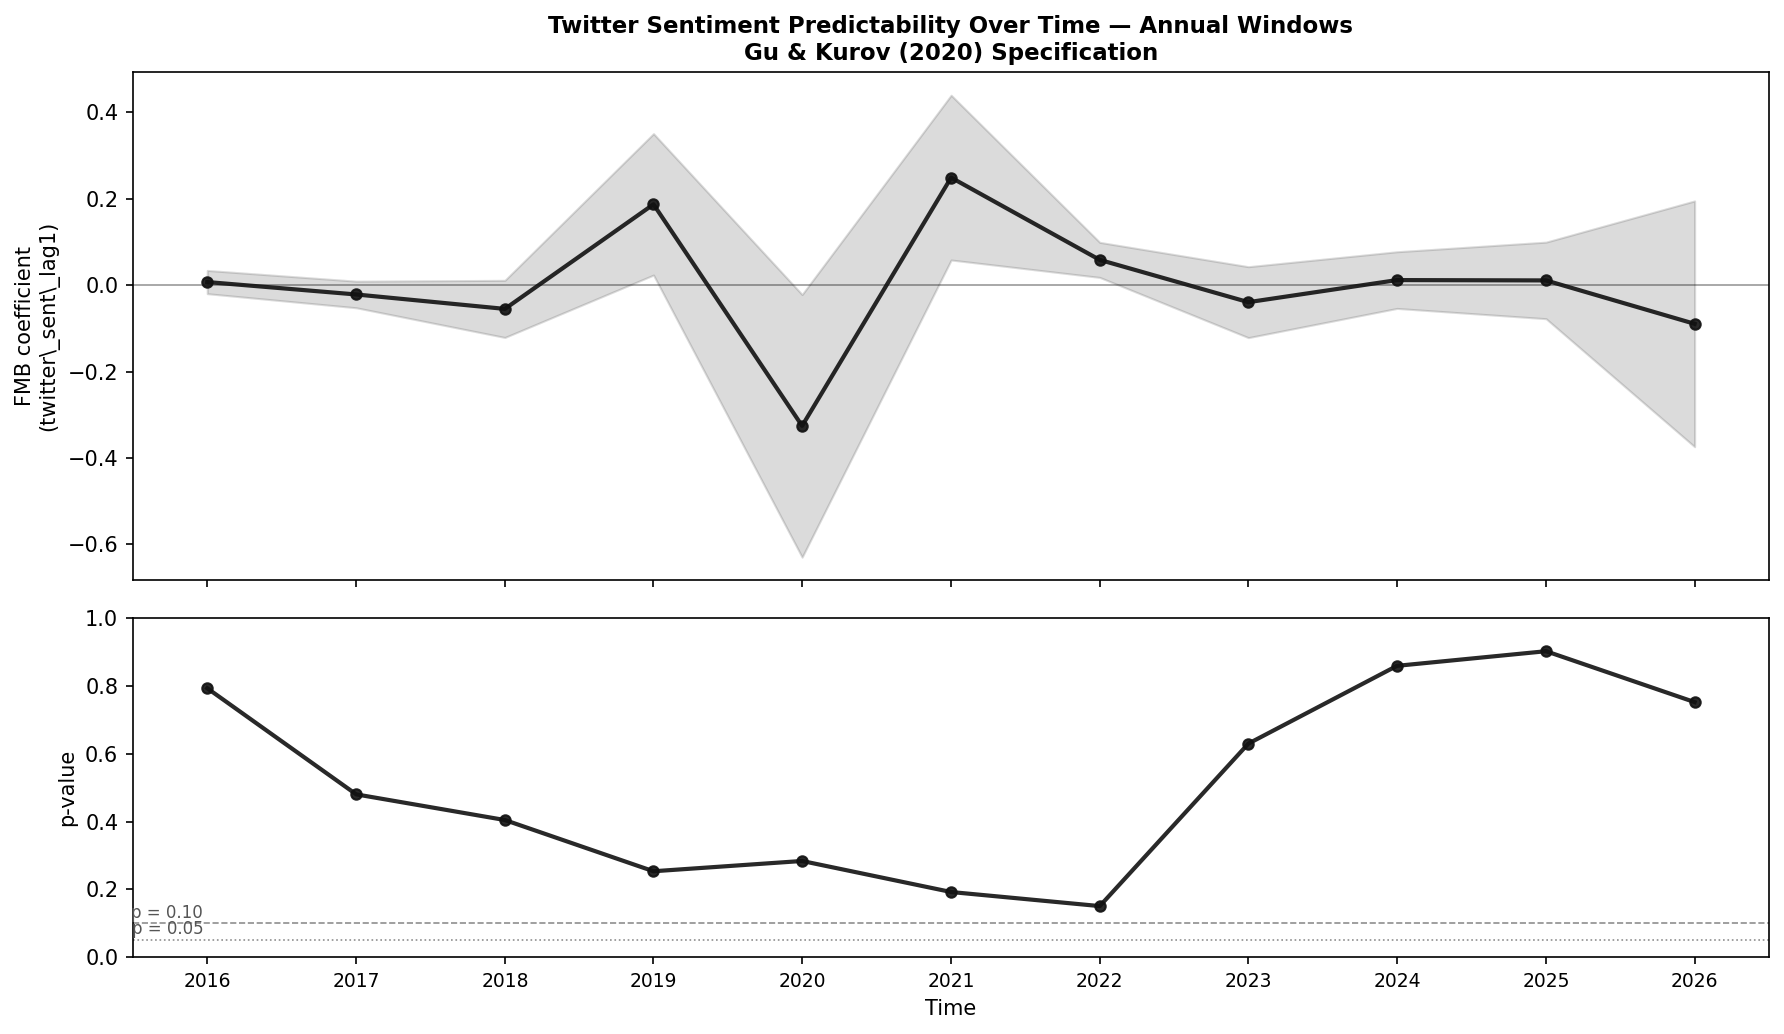
\includegraphics[width=\linewidth]{figures/gk_temporal_annual.png}
\caption{Twitter Sentiment Predictability Over Time --- Gu \& Kurov (2020) Specification (Annual windows). Top panel: Fama-MacBeth coefficient on \texttt{twitter\_sent\_lag1} with $\pm$1 SE band. Bottom panel: associated $p$-value; dashed lines at $p = 0.10$ and $p = 0.05$. Annual windows. Bandwidth = 5 lags; minimum cross-section $N = 30$.}
\label{fig:gk_temporal_annual}
\end{figure}

\begin{figure}[htbp]
\centering
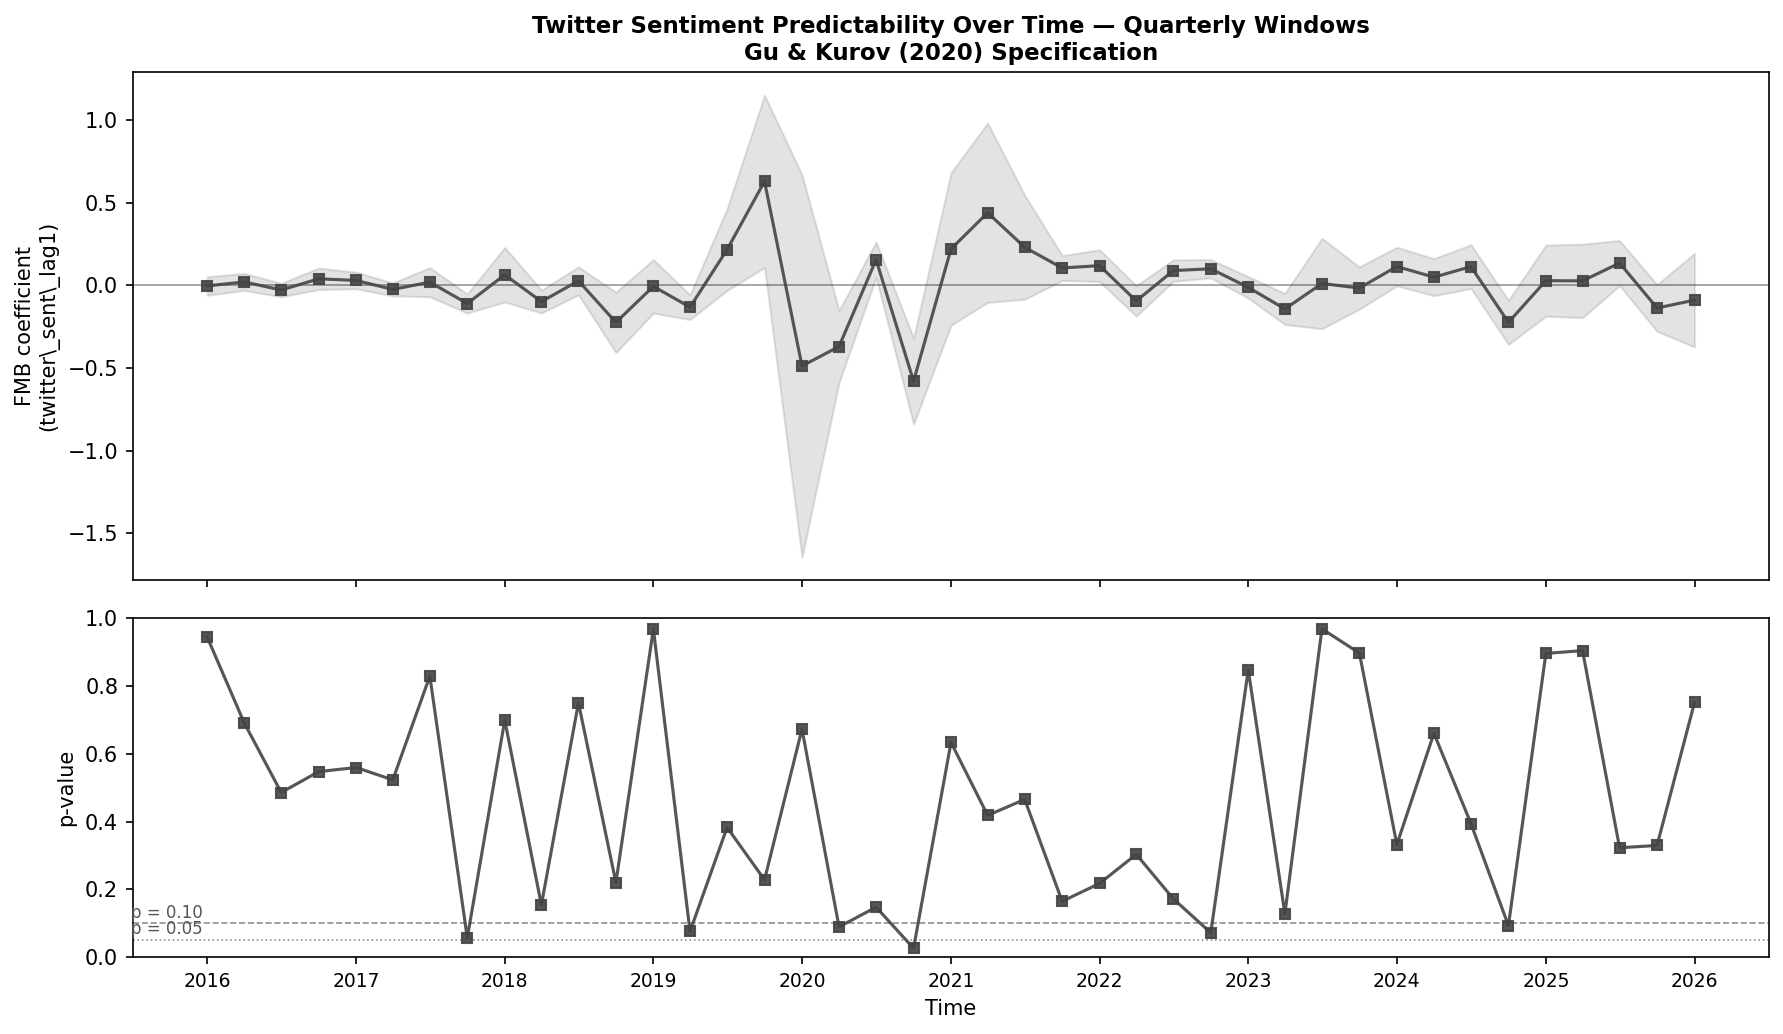
\includegraphics[width=\linewidth]{figures/gk_temporal_quarterly.png}
\caption{Twitter Sentiment Predictability Over Time --- Gu \& Kurov (2020) Specification (Quarterly windows). Top panel: Fama-MacBeth coefficient on \texttt{twitter\_sent\_lag1} with $\pm$1 SE band. Bottom panel: associated $p$-value; dashed lines at $p = 0.10$ and $p = 0.05$. Quarterly windows. Bandwidth = 4 lags; minimum cross-section $N = 20$.}
\label{fig:gk_temporal_quarterly}
\end{figure}

\begin{figure}[htbp]
\centering
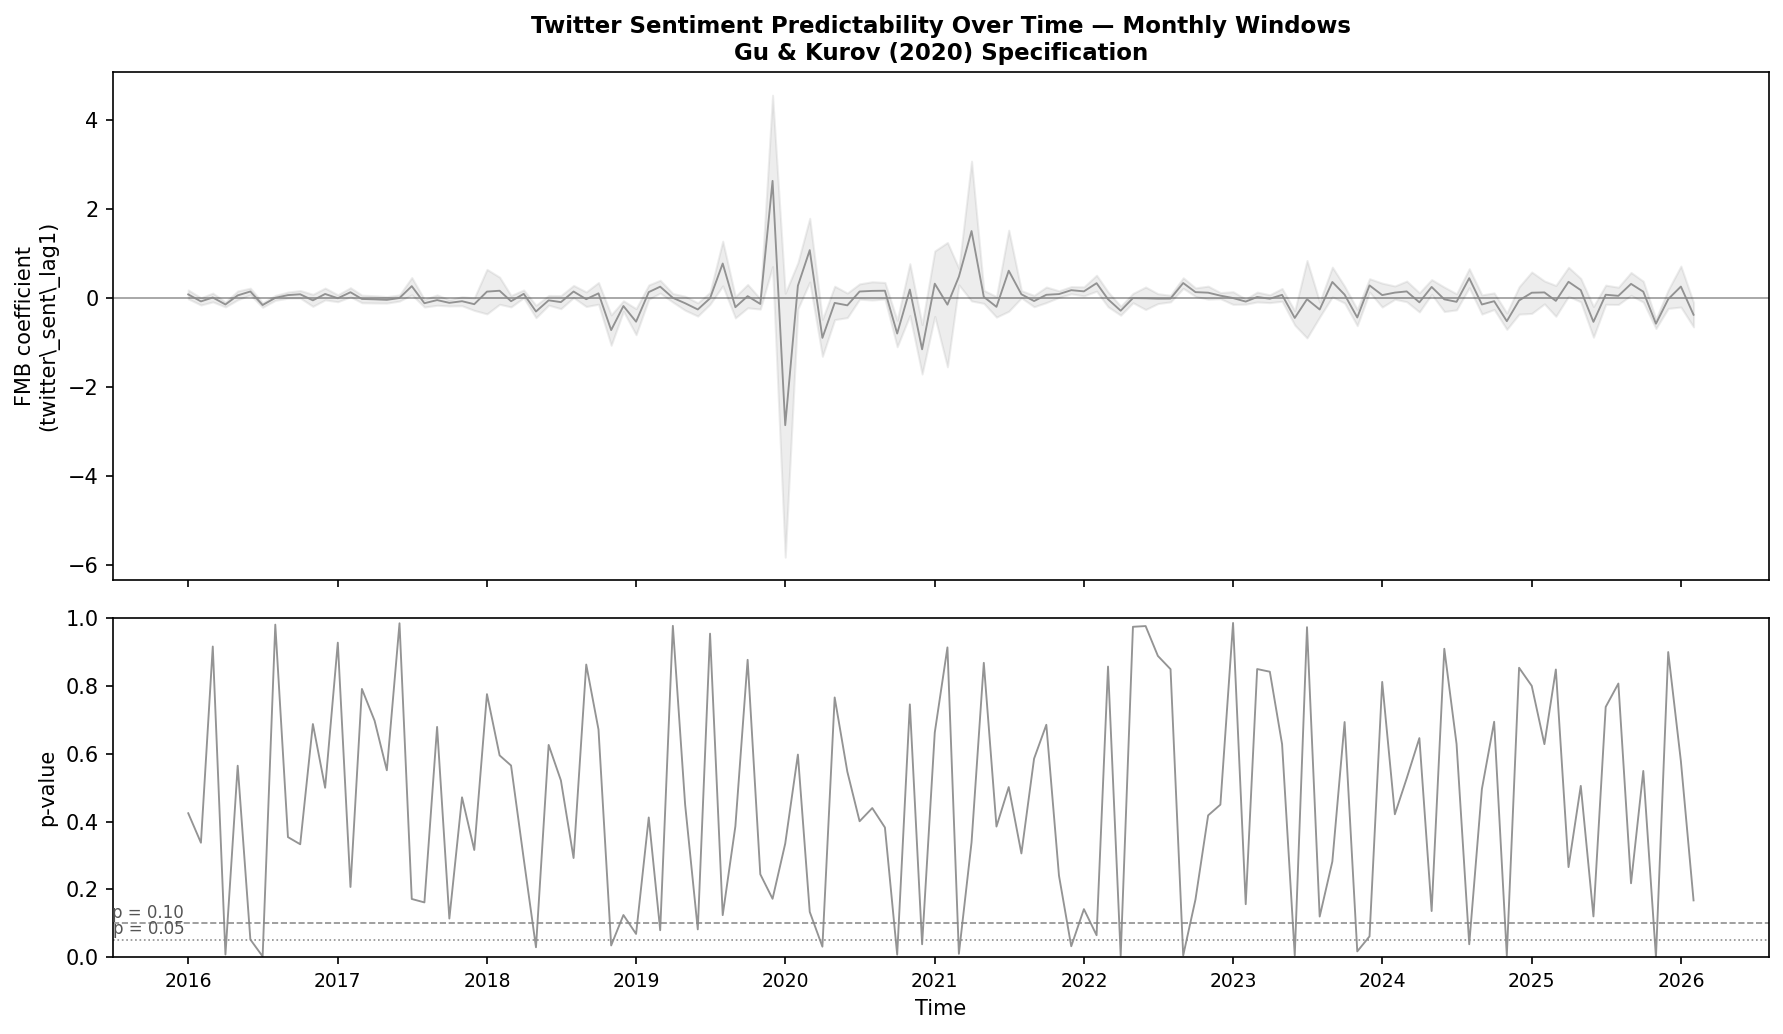
\includegraphics[width=\linewidth]{figures/gk_temporal_monthly.png}
\caption{Twitter Sentiment Predictability Over Time --- Gu \& Kurov (2020) Specification (Monthly windows). Top panel: Fama-MacBeth coefficient on \texttt{twitter\_sent\_lag1} with $\pm$1 SE band. Bottom panel: associated $p$-value; dashed lines at $p = 0.10$ and $p = 0.05$. Monthly windows. Bandwidth = 3 lags; minimum cross-section $N = 15$.}
\label{fig:gk_temporal_monthly}
\end{figure}

\subsection{Russell 3000: Cap-Group
Analysis}\label{russell-3000-cap-group-analysis}

Table~\ref{tab:russel_cap_ols}
reports Panel OLS results for the full Russell 3000 panel broken out by
cap group. The full-sample coefficient on \texttt{twitter\_sent} is
\(+ 0.708\) (\(p < 0.01\), \(N = 1,972,274\) firm-days)---positive and
significant, in contrast to the insignificant negative estimate in the
S\&P~500 panel. The sign difference reflects a fundamental difference in
the universe: the Russell 3000 includes roughly 2,500 mid- and small-cap
firms for which Twitter sentiment may carry informational content that
is already incorporated in S\&P~500 large-caps through more analyst and
formal media coverage, along with institutional investor flow which
purchases equities over time at fixed intervals.

The interaction specification (Model~2) includes
\(\text{twitter\_sent} \times \text{log\_mkt\_cap}\), estimated at
\(- 0.148\) (\(p < 0.10\)). The negative interaction coefficient implies
that the sentiment effect weakens as firm size increases, consistent
with the information-environment hypothesis. When the sample is
partitioned by cap group, the gradient is sharp: the large-cap
coefficient is \(+ 0.375\) (\(p < 0.01\)), the mid-cap coefficient is
\(+ 0.804\) (\(p < 0.01\)), and the small-cap coefficient is \(+ 0.942\)
(\(p < 0.01\)). The monotonic increase in magnitude from large to small
cap is consistent with declining marginal informational value of analyst
coverage: in large firms, Twitter provides little information
incremental to the dense institutional information set; in small firms,
a tweet may represent a critical information event.

Figure~\ref{fig:russel_temporal_annual} plots the full Russell 3000
Fama-MacBeth coefficient on \texttt{twitter\_sent\_lag1} by calendar
year. In contrast to the flat, uniformly insignificant S\&P~500 series
in Figure~\ref{fig:gk_temporal_annual}, the full Russell 3000 produces
positive and statistically significant estimates in most years, with
the effect strongest in 2018--2020. This confirms that the aggregate
signal driving the positive Panel OLS coefficient is real and
persistent over time, not an artifact of a particular sub-period.

\begin{figure}[htbp]
\centering
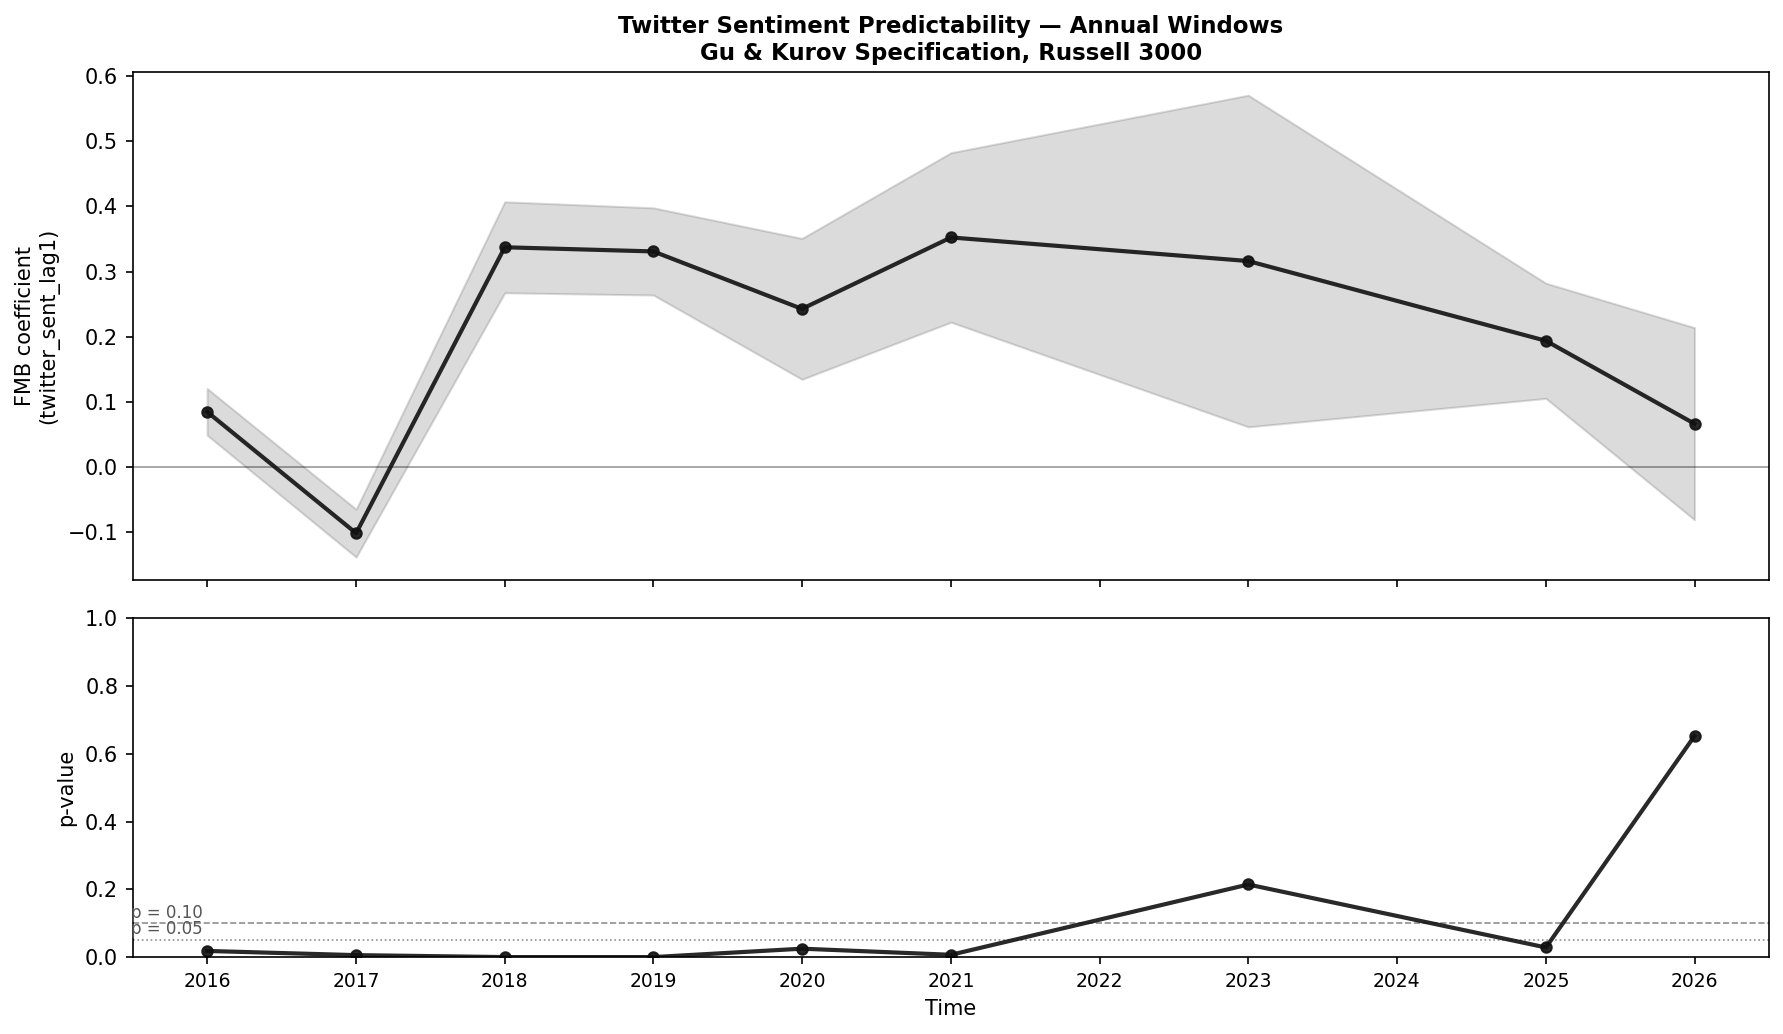
\includegraphics[width=\linewidth]{figures/russel_temporal_annual.png}
\caption{Twitter Sentiment Predictability --- Full Russell 3000 (Annual windows). Top panel: Fama-MacBeth coefficient on \texttt{twitter\_sent\_lag1} with $\pm$1 SE band. Bottom panel: associated $p$-value; dashed lines at $p = 0.10$ and $p = 0.05$. Annual windows. Bandwidth = 5 lags; minimum cross-section $N = 30$.}
\label{fig:russel_temporal_annual}
\end{figure}

The natural follow-up question is which firms drive this result.
Table~\ref{tab:russel_cap_fmb_annual}
reports Fama-MacBeth estimates by year and cap group. The gradient
across cap groups is consistent through time. Mid and small-cap
coefficients are statistically significant in most years (2016, 2018,
2019, 2020, 2021, 2025), while the large-cap series alternates between
significant and insignificant years with smaller point estimates. The
years 2018--2020 produce the strongest effects across all three groups,
coinciding with elevated retail trading activity in the lead-up to and
during the COVID-19 market episode. Two years (2022, 2024) are currently
under review due to possible data gaps in the Bloomberg feed and are
excluded from the tabular summary; the temporal figure includes these
years where sufficient cross-sectional observations are available.

Figure~\ref{fig:russel_cap_temporal_annual}
plots the three cap-group series together. The visual contrast is clear:
the mid and small-cap lines track at substantially higher coefficient
levels with more consistent statistical significance, while the
large-cap line hovers near zero with wide confidence bands in most
years. This figure represents the central result of the Russell 3000
extension.

\textbf{Long-short observation.} The daily long-short portfolio---long
top-decile, short bottom-decile sentiment firms---generates positive
returns across most years in the Russell 3000 sample, including during
years when the Fama-MacBeth regression coefficient is modest. This
coexistence of a weak aggregate coefficient with positive long-short
performance suggests that the sentiment signal is concentrated in the
tails of the cross-sectional distribution, producing a tradeable spread
even when the full-cross-section average is near zero. A full Sharpe
analysis by cap group is forthcoming pending calibration of the return
computation.

\begin{figure}[htbp]
\centering
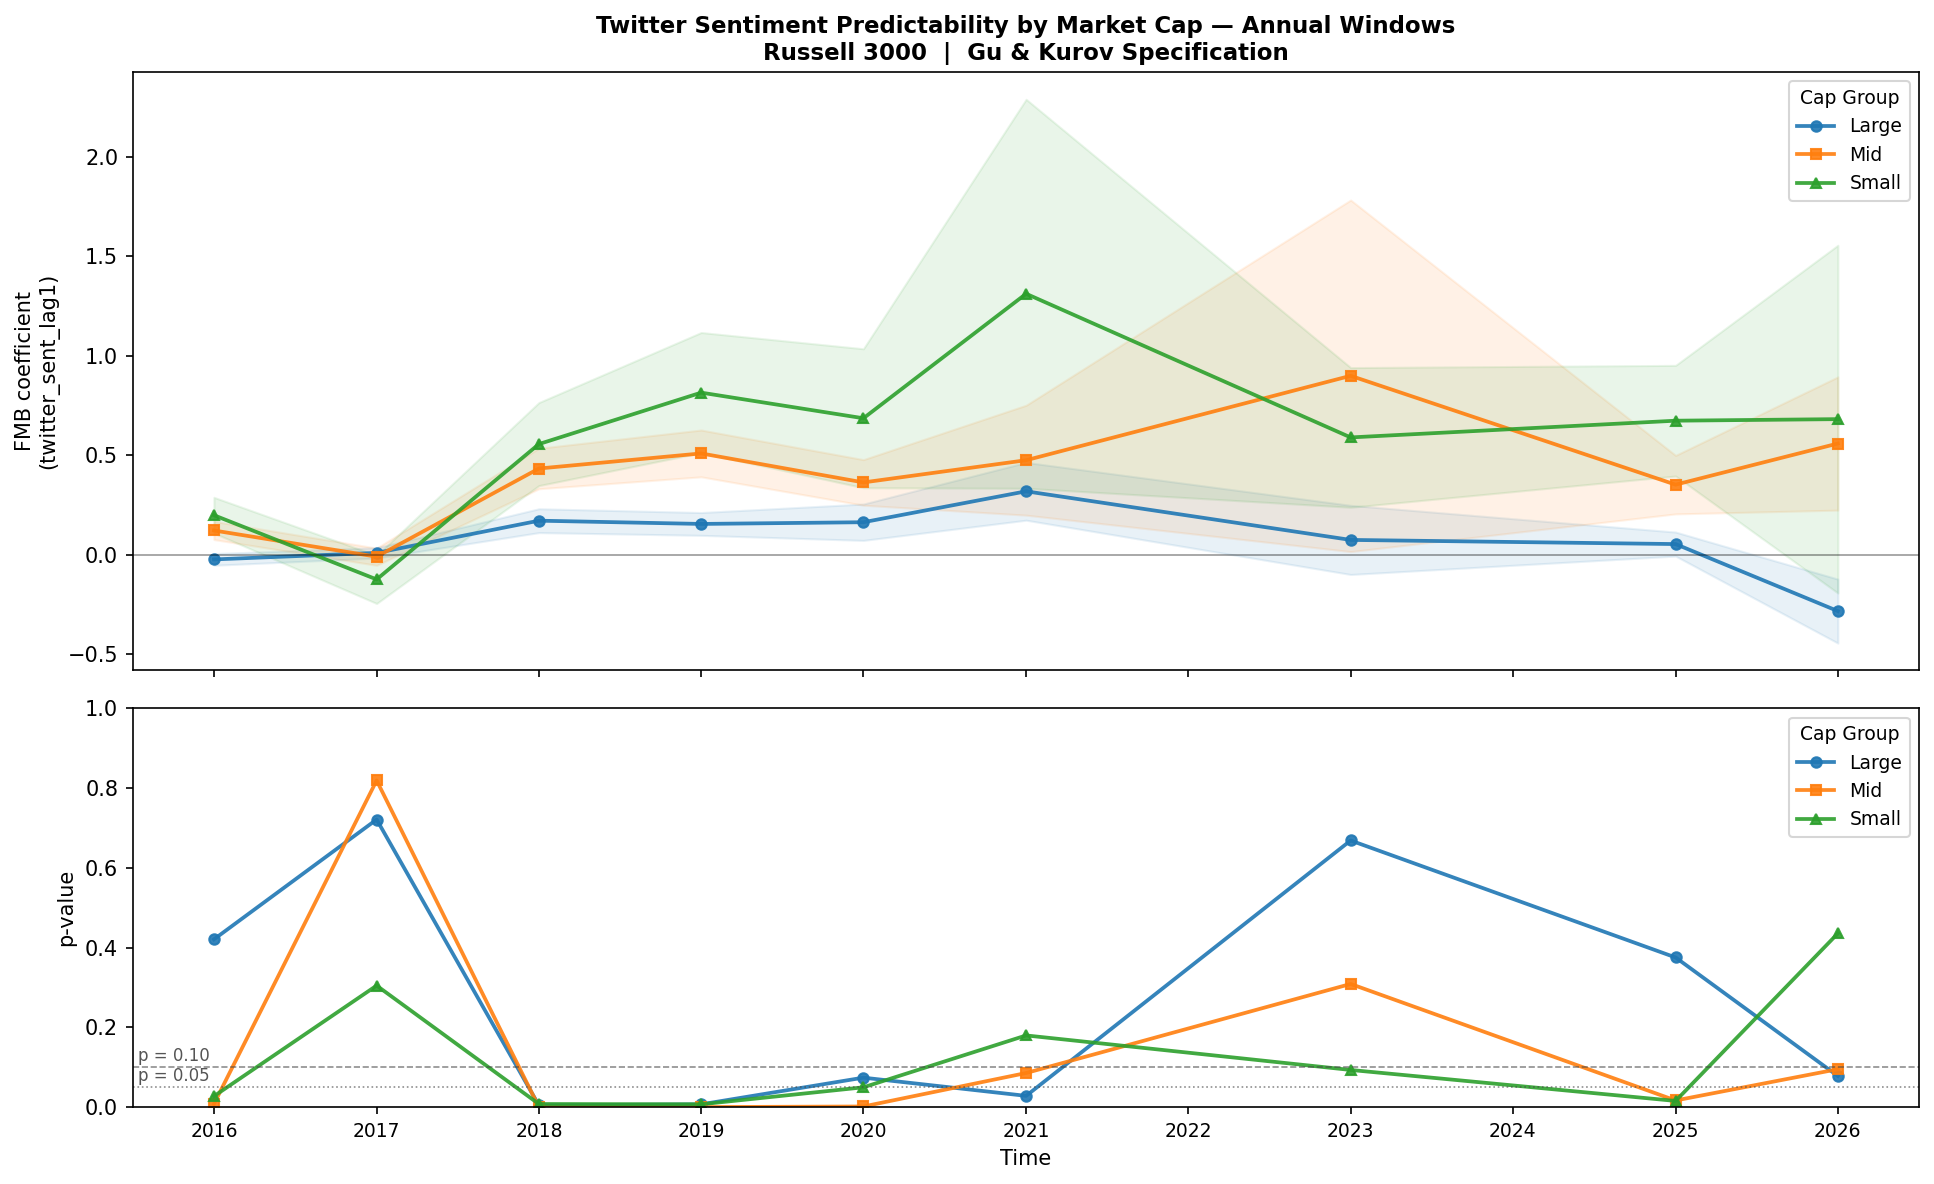
\includegraphics[width=\linewidth]{figures/russel_cap_temporal_annual.png}
\caption{Twitter Sentiment Predictability by Market Cap --- Russell 3000 (Annual windows). Top panel: Fama-MacBeth coefficient on \texttt{twitter\_sent\_lag1} with $\pm$1 SE band for large (blue), mid (orange), and small (green) cap firms. Bottom panel: $p$-values; dashed lines at $p = 0.10$ and $p = 0.05$. Annual windows. Bandwidth = 5 lags; minimum cross-section $N = 20$ per group.}
\label{fig:russel_cap_temporal_annual}
\end{figure}

\begin{figure}[htbp]
\centering
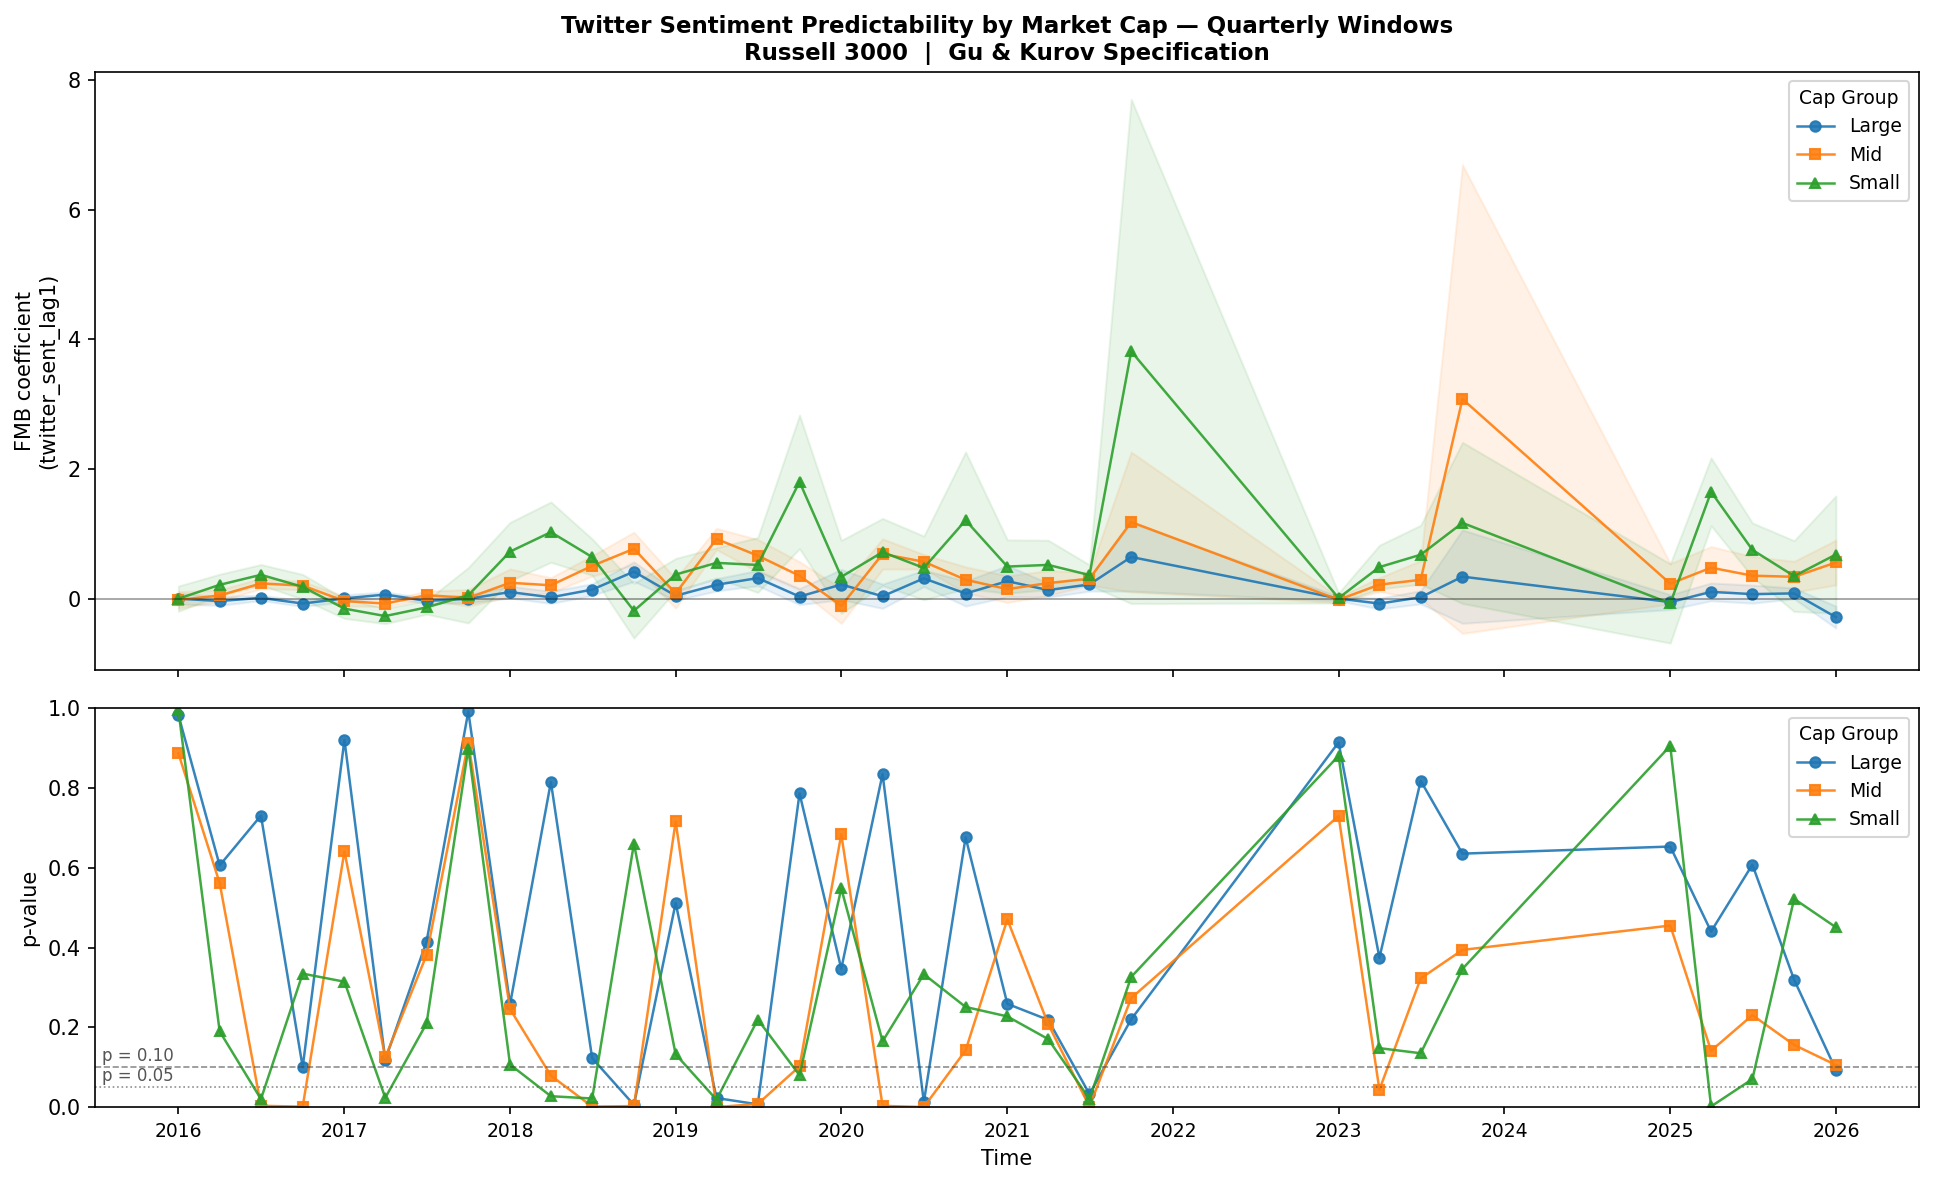
\includegraphics[width=\linewidth]{figures/russel_cap_temporal_quarterly.png}
\caption{Twitter Sentiment Predictability by Market Cap --- Russell 3000 (Quarterly windows). Top panel: Fama-MacBeth coefficient on \texttt{twitter\_sent\_lag1} with $\pm$1 SE band for large (blue), mid (orange), and small (green) cap firms. Bottom panel: $p$-values; dashed lines at $p = 0.10$ and $p = 0.05$. Quarterly windows. Bandwidth = 4 lags; minimum cross-section $N = 15$ per group.}
\label{fig:russel_cap_temporal_quarterly}
\end{figure}
